% C.4 邻补角与角平分线：OD 平分 ∠AOB，OE 平分 ∠BOC
\documentclass[tikz,border=4pt]{standalone}
\usepackage{ctex}
\usepackage{amsmath}
\usetikzlibrary{calc, arrows.meta}
\begin{document}
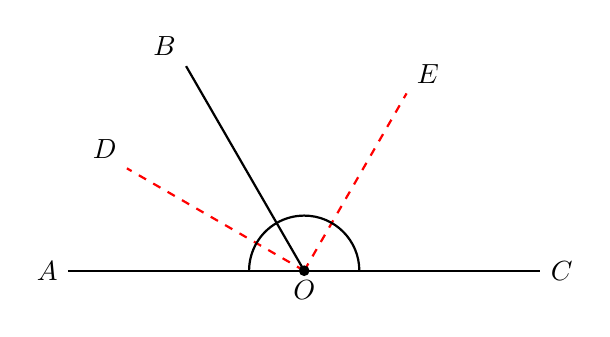
\begin{tikzpicture}[scale=1.0, thick]
  \coordinate (O) at (0,0);
  \pgfmathsetmacro{\angAOB}{120}
  \coordinate (A) at (-3,0);
  \coordinate (C) at (3,0);
  \coordinate (B) at ({3*cos(\angAOB)}, {3*sin(\angAOB)});
  \coordinate (D) at ({2.6*cos(\angAOB/2+90)}, {2.6*sin(\angAOB/2+90)})  ; % bisector of AOB: from 180 to 120 → mid 150
  \coordinate (D) at ({2.6*cos(150)}, {2.6*sin(150)});
  \coordinate (E) at ({2.6*cos(60)}, {2.6*sin(60)});
  \draw (A) -- (C);
  \draw (O) -- (B);
  \draw[red, dashed] (O) -- (D);
  \draw[red, dashed] (O) -- (E);
  \filldraw (O) circle (1.5pt);
  \node[left] at (A) {$A$};
  \node[right] at (C) {$C$};
  \node[above left] at (B) {$B$};
  \node[above left] at (D) {$D$};
  \node[above right] at (E) {$E$};
  \node[below] at (O) {$O$};
  % 角弧
  \draw (0.7,0) arc (0:\angAOB:0.7);
  \draw ({0.7*cos(\angAOB)},{0.7*sin(\angAOB)}) arc (\angAOB:180:0.7);
\end{tikzpicture}
\end{document}
